\documentclass{beamer}
\usetheme{Frankfurt}

\usepackage{listings}

\newcommand{\todo}[1]{\alert{TODO #1}}

\title{Networking/OS}
\subtitle{Lecture 2 \\ Computer Security DD2395}
\author[R. Guanciale]{
  Roberto Guanciale\\
  robertog@kth.se
}
\date{2015-11-04}
\begin{document}

\begin{frame}[plain]
  \titlepage
\end{frame}

\begin{frame}{Outline for Today}
  \begin{itemize}
    \item Computer networking
    \item Operating systems
  \end{itemize}
\end{frame}

\begin{frame}{Introduction to IP networking}
  \begin{itemize}
    \item An end host requests a web-page from a server via a local-area
      network
    \item The aim of this lecture is to give an overview of how this works
in practice
  \end{itemize}
  \begin{center}
    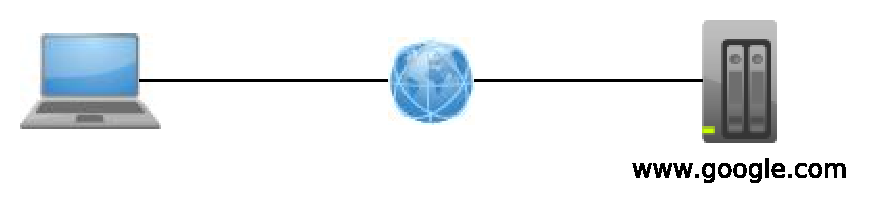
\includegraphics[width=0.5\linewidth]{net0}
  \end{center}
\end{frame}

\begin{frame}{Introduction to IP networking}
  Every routing domain is independently administrated
  \begin{center}
    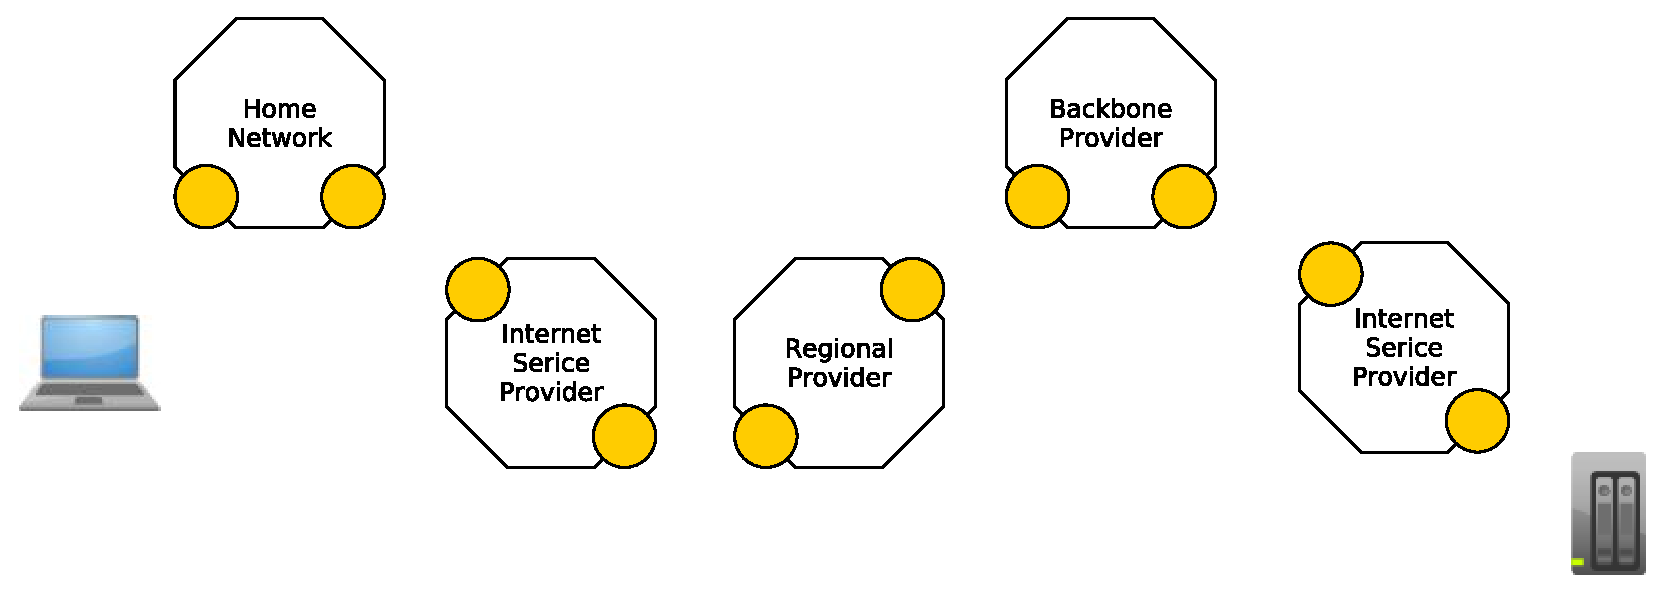
\includegraphics[width=0.8\linewidth]{net1}
  \end{center}
\end{frame}

\begin{frame}{The Hourglass Model}
  \begin{itemize}
    \item Anything over IP – IP over anything
    \item All applications depend on IP
    \item IP runs over all networks
    \item IP is at the heart of all communicati
  \end{itemize}
  \begin{center}
    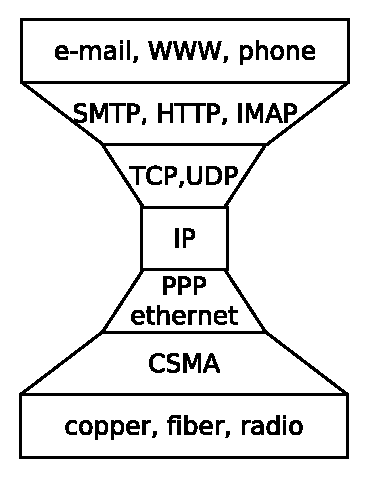
\includegraphics[width=0.4\linewidth]{net2}
  \end{center}
\end{frame}

\begin{frame}{Stack}
  \begin{center}
    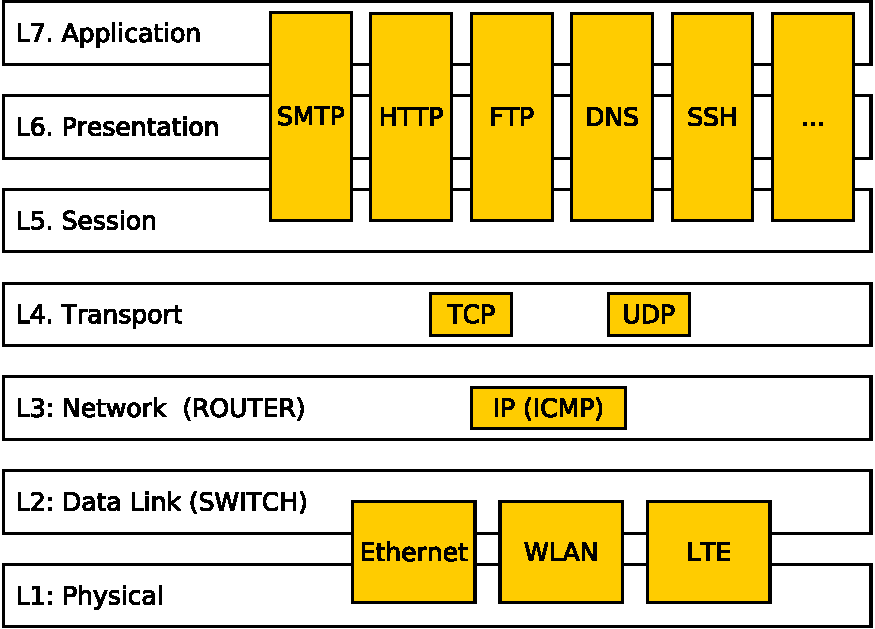
\includegraphics[width=0.4\linewidth]{stack}
  \end{center}
\end{frame}

\begin{frame}{Encapsulation}
  \begin{center}
    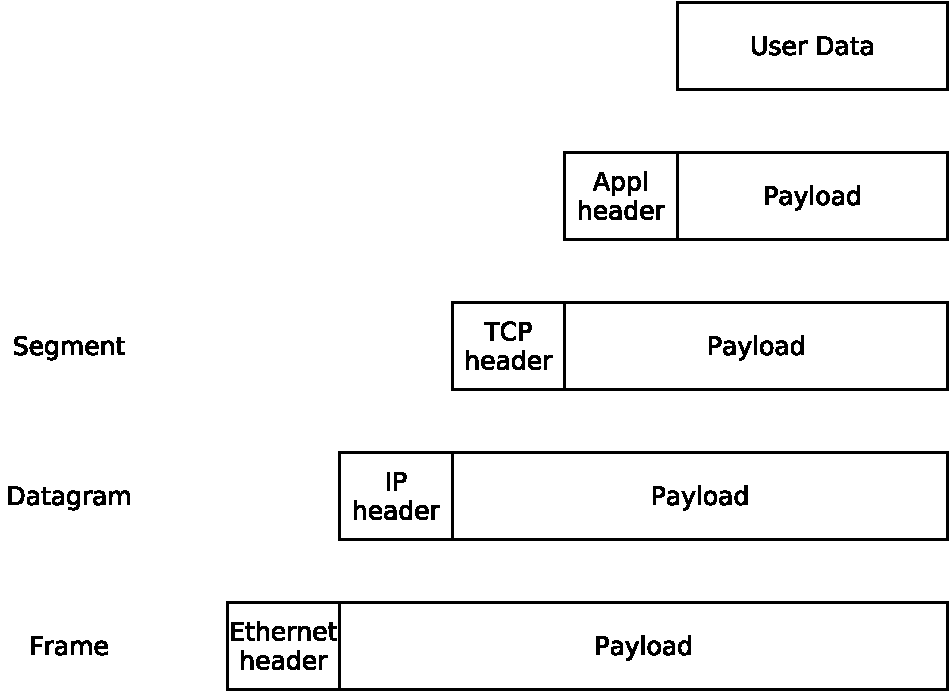
\includegraphics[width=0.7\linewidth]{encapsulation}
  \end{center}
\end{frame}

\begin{frame}
  \begin{itemize}
  \item Using a link-level protocol, you can now communicate
    directly over a link
  \item The network layer (IP) primarily adds the ability to cross
    several networks using 'routing'
  \item Each interface in an IPv4 Internet is assigned a unique 32-bit
internet address (Not node addresses!)
  \begin{itemize}
\item Address types
\item Unicast – one-to-one
\item Anycast - one-to-any
\item Multicast – one-to-many
\item Broadcast – one-to-all
  \end{itemize}
\item Notation, dotted-decimal: 192.36.125.18
\item An address has two purposes
  \begin{itemize}
\item Netid (prefix) identifies a network
\item Hostid identifies a node on that network
  \end{itemize}
\item Slash notation: 192.36.120.0/21
  \end{itemize}
\end{frame}

\begin{frame}{IP-header}
  \begin{center}
    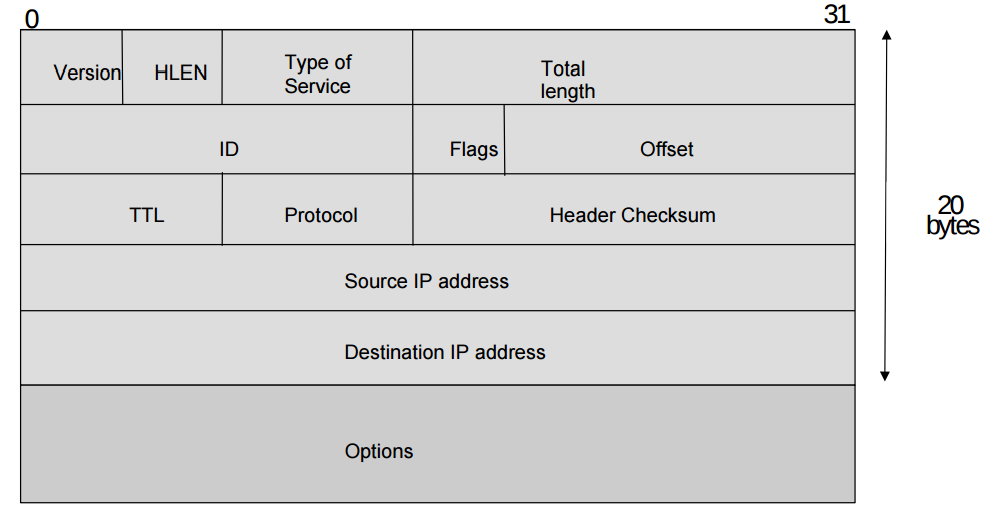
\includegraphics[width=0.9\linewidth]{IP-header}
  \end{center}
\end{frame}

\begin{frame}{IP-routing}
  \begin{center}
    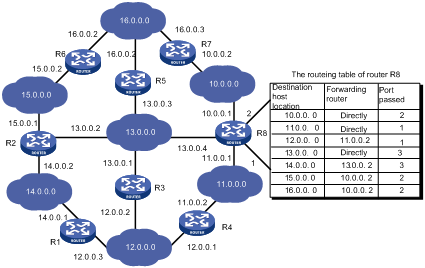
\includegraphics[width=0.9\linewidth]{table}
  \end{center}
\end{frame}

\begin{frame}{ICMP}
  \begin{itemize}
  \item ICMP is a limited signalling protocol for IPv4.
  \item Report IP problems back to sender
  \item Control and Management
  \item 0 - Echo reply (used to ping)
  \item 3 - Destination Unreachable
  \item 8 - Echo request (used to ping)
  \item 9 - Router Advertisement
  \item 11 - Time Exceeded[
  \item 13 - Timestamp
  \item 14 - Timestamp Reply
  \item \dots
  \end{itemize}
\end{frame}

\begin{frame}{Transport layer}
  \begin{itemize}
  \item Provides service to end-applications: ports
  \item UDP
    \begin{itemize}
      \item Packet-oriented
      \item Unreliable
      \item Full-duplex
      \item Data in packets
      \item Real-time traffic/Reliability in application
    \end{itemize}
  \item TCP
    \begin{itemize}
      \item Connection-oriented
      \item Reliable
      \item Full-duplex
      \item Data as byte-stream
      \item Mostly used
    \end{itemize}
  \end{itemize}
\end{frame}

\begin{frame}{UDP}
    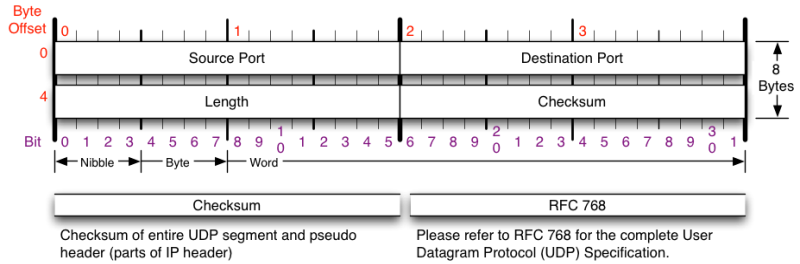
\includegraphics[width=0.9\linewidth]{udp}
\end{frame}

\begin{frame}{TCP}
    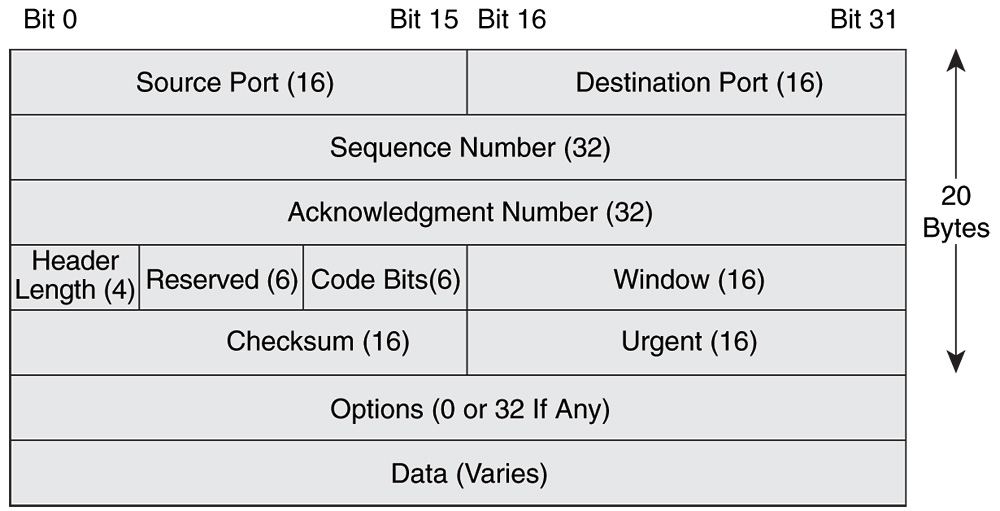
\includegraphics[width=0.9\linewidth]{tcp}
\end{frame}

\begin{frame}{TCP}
    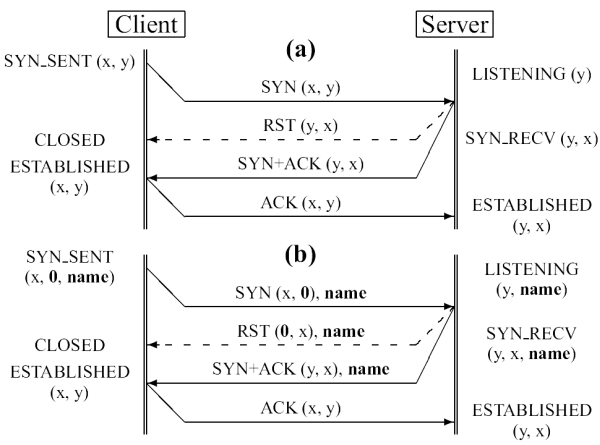
\includegraphics[width=0.7\linewidth]{synack}
\end{frame}

\begin{frame}{DNS}
\begin{itemize}
  \item Why do we need names?
  \item In the underlying network and transport layers it is all about
addresses.
\item Names are better for humans\\
fe80::216:d3ff:fecc:c00d
\item Names add another layer of indirection
\begin{itemize}
\item One name can map to several logical addresses
\item One logical adress can map to several names
\item Names can be used for other things than just addressing
  load balancing, mail direction, descriptions, finding services,
\end{itemize}
\end{itemize}
\end{frame}

\begin{frame}{DNS architecture}
\begin{itemize}
  \item Names are structured hierarchically - in a tree form
  \item The DNS architecture is client-server
\begin{itemize}
\item Client is called resolver
\item Server is called name server
\end{itemize}
\item The resolver queries the nameservers hierarchically
\item Protocol over UDP
\end{itemize}
\end{frame}

\begin{frame}{SMTP}
    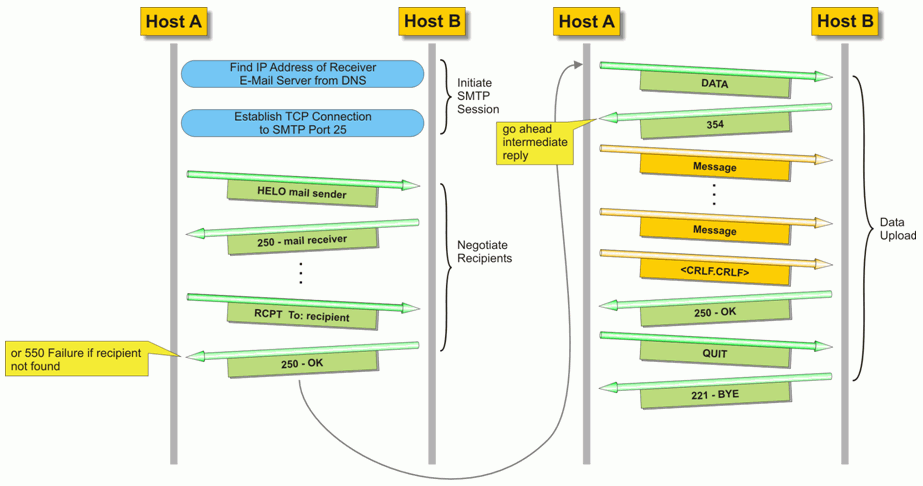
\includegraphics[width=0.7\linewidth]{smtp}
\end{frame}
\begin{frame}{SMTP}
    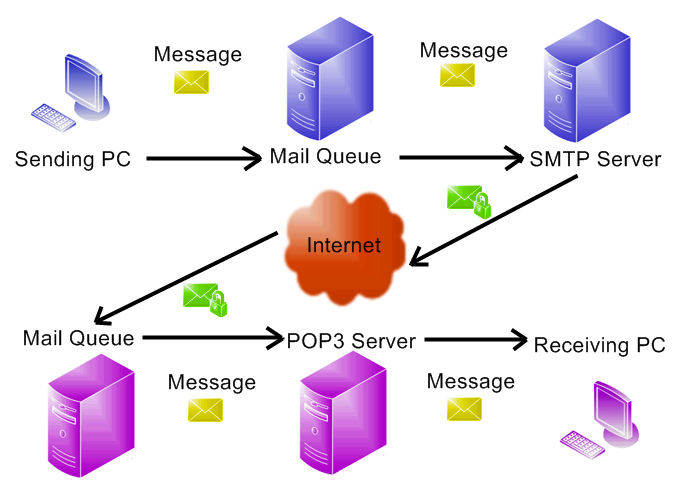
\includegraphics[width=0.7\linewidth]{smrp_queue}
\end{frame}
\begin{frame}{SMTP}
    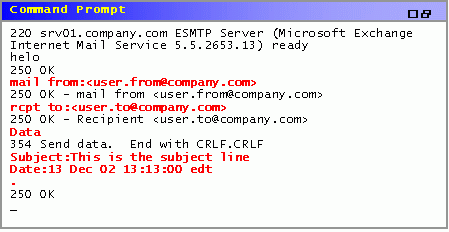
\includegraphics[width=0.7\linewidth]{smtp_shell}
\end{frame}
\begin{frame}{HTTP}
    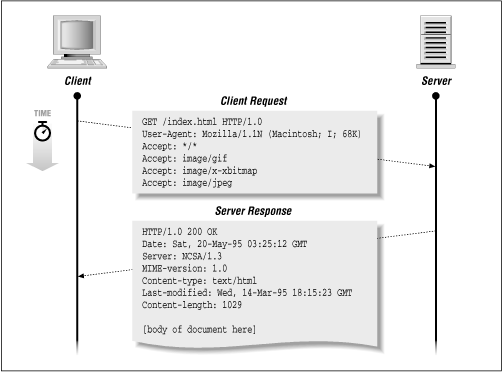
\includegraphics[width=0.7\linewidth]{http}
\end{frame}


\end{document}
